\documentclass[12pt,fleqn]{article}\usepackage{../common}
\begin{document}
Esle-Indirge Mimarisi (Map-Reduce Architecture)

Bu kavrami bir veri analiz isini iki evreye ayirir. Bunlardan birincisi
Esleme evresinde, ki bu evrede eline gecen veri parcasini alan her analiz
servisi (ki bunlardan pek cok var, farkli makinalarda), surecler
kendilerine verilen dosyaya bakarak anahtar-deger ikilileri
uretirler. Kelime sayma ornegi icin bu anahtarlar kelimeler, sayilar ise
hep 1. Mesela "A A B" icin tek bir esleyici A: 1, A: 1, B: 1 uretir.

Bir sonraki evre, indirgeme evresinde, her servisten alinan anahtarlardaki
degerler "birlestirilir" yani daha aza "indirgenir". Fakat dikkat:
birlestirme denince tek bir nihai servisin her seyi tek basina indirgedigi
zannedilmesin. Indirgeme evresi de birden fazla makinada isleyebilir.

Anahtarlar birlestirme "birimini" olustururlar [1]. Indirgeme islemi ise
iki, uc hatta birden fazla girdiyi isleyebilecek turden bir kod
olmalidir. Fakat zaten kelime sayma problemin ozunde zaten bu vardir,
hersey ayri ayri, parca parca toplanabilir, bir Indirgeyici iki eslenmis
dosya aliyor diyelim, biri A: 1, A: 1, B: 1, digeri A: 1, B:1; bunlari A:
3, B: 2 olarak indirgeyebilir / birlestirebiliriz.  Diger makinalarda
baskalari baska veriler almistir, onlar kendi caplarinda kendi
birlestirimlerini yapmaktadirlar. Indirgeme ve yuk dagitim birimi
anahtardir, indirgeme safhasinda mesela A anahtari tek bir makinaya
gonderilecektir, o anahtarin birlesiminden o makina sorumlu olacaktir.

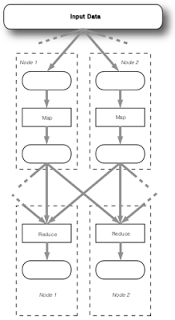
\includegraphics[height=12cm]{mr.png}

Isin mekanigine bakinca oldukca basit gibi gelebilir. Fakat sasirtici kadar
cok analiz islemi ustteki sekilde temsil edilebilmektedir ve sonuc olarak
paralelize edilebilmektedir. Tabii isin mekanigi derken sadece anahtarlara
ayirmaktan bahsetmiyoruz, analiz isleminin, her ne ise, "azar azar, ayri
ayri ust uste koya koya sonuca ilerleyebilecek" sekilde tekrar tasarlanmasi
gerekiyor. Kelime toplama, hatta toplama niye burada uygun goruyoruz,
2,3,4,5 eklerlerken 2+3=5,4+5=9 ardindan 5+9=14 elde edebiliriz, ama diger
bir sekilde 3+4=7,2+5=7 arkasindan tekrar 7+7=14 yani ayni sonucu elde
edebiliyoruz. Toplama isleminin ruhunda "siradan bagimsiz olmak" var, ve bu
bagimsizlik paralelize etmekte isimize yariyor.

Hadoop ile Patent Verisi Islemek

75-99 yillari arasinda hangi patentin hangi hangi patentlere referans
verdigi ve patentler hakkinda detayli verileri Hadoop ile
isleyecegiz. Veriler alttaki baglantidan alinabilir, gerekli dosyalar
Dosyalar \verb!cite75_99.txt! ve \verb!apat63_99.txt!. Bu dosyalari
acip biz diyelim ki \verb!/data! altina koyduk. 

\verb!www.nber.org/patents/!

Referans verisine bakarsak,

\begin{minted}[fontsize=\footnotesize]{python}
!head -10 /data/cite75_99.txt
\end{minted}

\begin{verbatim}
"CITING","CITED"
3858241,956203
3858241,1324234
3858241,3398406
3858241,3557384
3858241,3634889
3858242,1515701
3858242,3319261
3858242,3668705
3858242,3707004
\end{verbatim}

Bu veri, hangi patentin hangi diger patenti kullandigini "tek" patent
bazinda gostermekte. Detayli patent verisine bakalim

\begin{minted}[fontsize=\footnotesize]{python}
!head -10 /data/apat63_99.txt
\end{minted}

\begin{verbatim}
"PATENT","GYEAR","GDATE","APPYEAR","COUNTRY","POSTATE","ASSIGNEE","ASSCODE","CLAIMS","NCLASS","CAT","SUBCAT","CMADE","CRECEIVE","RATIOCIT","GENERAL","ORIGINAL","FWDAPLAG","BCKGTLAG","SELFCTUB","SELFCTLB","SECDUPBD","SECDLWBD"
3070801,1963,1096,,"BE","",,1,,269,6,69,,1,,0,,,,,,,
3070802,1963,1096,,"US","TX",,1,,2,6,63,,0,,,,,,,,,
3070803,1963,1096,,"US","IL",,1,,2,6,63,,9,,0.3704,,,,,,,
3070804,1963,1096,,"US","OH",,1,,2,6,63,,3,,0.6667,,,,,,,
3070805,1963,1096,,"US","CA",,1,,2,6,63,,1,,0,,,,,,,
3070806,1963,1096,,"US","PA",,1,,2,6,63,,0,,,,,,,,,
3070807,1963,1096,,"US","OH",,1,,623,3,39,,3,,0.4444,,,,,,,
3070808,1963,1096,,"US","IA",,1,,623,3,39,,4,,0.375,,,,,,,
3070809,1963,1096,,"US","AZ",,1,,4,6,65,,0,,,,,,,,,
\end{verbatim}

Simdi patent detay verisinden bir orneklem (sample) alalim. Daha ufak bir
veri kumesiyle calismak ilk basta faydali olabilir, gelistirme test etme
surecini hizlandirir.

\begin{minted}[fontsize=\footnotesize]{python}
!chmod a+r /data/apat63_99.txt
!head -1 /data/apat63_99.txt > /data/apat63_99_sampled.txt
!cat /data/apat63_99.txt | perl -n -e 'print if (rand() < .05)' >> /data/apat63_99_sampled.txt
\end{minted}

Hadoop baslatalim

\begin{minted}[fontsize=\footnotesize]{python}
!ssh localhost -l hduser /home/hduser/Downloads/hadoop*/bin/stop-all.sh
!ssh localhost -l hduser /home/hduser/Downloads/hadoop*/bin/start-all.sh
\end{minted}

\begin{verbatim}
no jobtracker to stop
localhost: no tasktracker to stop
no namenode to stop
localhost: no datanode to stop
localhost: no secondarynamenode to stop
starting namenode, logging to /home/hduser/Downloads/hadoop-1.0.4/libexec/../logs/hadoop-hduser-namenode-burak-Aspire-S3.out
localhost: starting datanode, logging to /home/hduser/Downloads/hadoop-1.0.4/libexec/../logs/hadoop-hduser-datanode-burak-Aspire-S3.out
localhost: starting secondarynamenode, logging to /home/hduser/Downloads/hadoop-1.0.4/libexec/../logs/hadoop-hduser-secondarynamenode-burak-Aspire-S3.out
starting jobtracker, logging to /home/hduser/Downloads/hadoop-1.0.4/libexec/../logs/hadoop-hduser-jobtracker-burak-Aspire-S3.out
localhost: starting tasktracker, logging to /home/hduser/Downloads/hadoop-1.0.4/libexec/../logs/hadoop-hduser-tasktracker-burak-Aspire-S3.out
\end{verbatim}

\begin{minted}[fontsize=\footnotesize]{python}
/home/hduser/Downloads/hadoop*/bin/hadoop dfs -mkdir /user/hduser/patent
!ssh localhost -l hduser /home/hduser/Downloads/hadoop*/bin/hadoop \
dfs -ls /user/hduser/patent
\end{minted}

\begin{verbatim}
Found 2 items
-rw-r--r--   1 hduser supergroup ...  /user/hduser/patent/apat63_99.txt
-rw-r--r--   1 hduser supergroup ...   /user/hduser/patent/apat63_99_sampled.txt
\end{verbatim}

\begin{minted}[fontsize=\footnotesize]{python}
!ssh localhost -l hduser /home/hduser/Downloads/hadoop*/bin/hadoop \
dfs -copyFromLocal /data/apat63_99_sampled.txt \
/user/hduser/patent/apat63_99_sampled.txt
\end{minted}

\begin{verbatim}
copyFromLocal: Target /user/hduser/patent/apat63_99_sampled.txt already exists
\end{verbatim}

Amacimiz patent verisindeki ulke (country) kodunu kullanarak her ulke
basina ortalama ne kadar patent uretildigini
hesaplamak. Esleme-Indirgeme (Map-Reduce) dongusunde esleme kismini
yapacak program asagida.

\begin{minted}[fontsize=\footnotesize]{python}
#!/usr/bin/python
import os,sys
os.environ['MPLCONFIGDIR']='/tmp' 
import pandas as pd
data = pd.read_csv(sys.stdin,sep=",",index_col=0,usecols=[0,4,8])
df = data[pd.notnull(data.ix[:,0]) \& pd.notnull(data.ix[:,1])].ix[:,0:2]
df.to_csv(sys.stdout,sep="\t",index=False,header=False)
\end{minted}

Indirgeyici yazmadan once programimizi iki sekilde test edelim. Bu
sekillerden birisi hic indirgeyici olmadan, ikincisi
\verb!IdentityReducer! denen kendisine gecilen veriyi oldugu
gibi disari atan (ama yine de ortada bir indirgeyici oldugu icin
sonradan bazi islemlerin yine de yapildigi) seklinde. Bu iki kullanim
Hadoop kodlarinda hata bulma / temizleme icin faydali olabiliyor.

\begin{minted}[fontsize=\footnotesize]{python}
!cp mapper.py /tmp/
!chmod a+r /tmp/mapper.py
!chmod a+x /tmp/mapper.py
\end{minted}

\begin{minted}[fontsize=\footnotesize]{python}
!ssh localhost -l hduser /home/hduser/Downloads/hadoop*/bin/hadoop \
dfs -rmr /user/hduser/output
!ssh localhost -l hduser /home/hduser/Downloads/hadoop*/bin/hadoop \
jar \$HOME/Downloads/hadoop*/contrib/streaming/hadoop-*streaming*.jar\
-input patent/apat63_99_sampled.txt  -output output  \
-mapper /tmp/mapper.py -numReduceTasks 0 
\end{minted}

\begin{verbatim}
Deleted hdfs://localhost:54310/user/hduser/output
packageJobJar: [/app/hadoop/tmp/hadoop-unjar2555196345671652661/] [] /tmp/streamjob5013687273729997973.jar tmpDir=null
13/02/24 16:30:26 INFO util.NativeCodeLoader: Loaded the native-hadoop library
13/02/24 16:30:26 WARN snappy.LoadSnappy: Snappy native library not loaded
13/02/24 16:30:26 INFO mapred.FileInputFormat: Total input paths to process : 1
13/02/24 16:30:27 INFO streaming.StreamJob: getLocalDirs(): [/app/hadoop/tmp/mapred/local]
13/02/24 16:30:27 INFO streaming.StreamJob: Running job: job_201302241611_0012
13/02/24 16:30:27 INFO streaming.StreamJob: To kill this job, run:
13/02/24 16:30:27 INFO streaming.StreamJob: /home/hduser/Downloads/hadoop-1.0.4/libexec/../bin/hadoop job  -Dmapred.job.tracker=localhost:54311 -kill job_201302241611_0012
13/02/24 16:30:27 INFO streaming.StreamJob: Tracking URL: http://localhost:50030/jobdetails.jsp?jobid=job_201302241611_0012
13/02/24 16:30:28 INFO streaming.StreamJob:  map 0%  reduce 0%
13/02/24 16:30:43 INFO streaming.StreamJob:  map 100%  reduce 0%
13/02/24 16:30:49 INFO streaming.StreamJob:  map 100%  reduce 100%
13/02/24 16:30:49 INFO streaming.StreamJob: Job complete: job_201302241611_0012
13/02/24 16:30:49 INFO streaming.StreamJob: Output: output
\end{verbatim}

\begin{minted}[fontsize=\footnotesize]{python}
!ssh localhost -l hduser /home/hduser/Downloads/hadoop*/bin/hadoop dfs  -copyToLocal output /tmp/
!head -20 /tmp/output/part-00000
\end{minted}

\begin{verbatim}
AD	14.0
AE	15.4
AG	13.25
AI	10.0
AM	18.0
AN	9.625
AR	9.188990825688073
AT	10.683988393563704
AU	12.291563832174107
AW	15.5
AZ	11.0
BB	11.0
BE	11.945544554455445
BG	4.9899497487437188
BH	6.5
BM	10.076923076923077
BN	9.0
BO	11.75
BR	9.358426966292134
BS	15.778846153846153
\end{verbatim}

Ustteki sonucta goruyoruz ki anahtarlar uretilmis, ama ciktilar
anahtara gore siralanmamislar. Hatta ustteki sira girdi sirasiyla
tipatip ayni. Simdi \verb!IdentityReducer! uzerinden.

\begin{minted}[fontsize=\footnotesize]{python}
!ssh localhost -l hduser /home/hduser/Downloads/hadoop*/bin/hadoop \
dfs -rmr /user/hduser/output
!ssh localhost -l hduser /home/hduser/Downloads/hadoop*/bin/hadoop \
 jar /home/hduser/Downloads/hadoop*/contrib/streaming/hadoop-*streaming*.jar \
 -input patent/apat63_99_sampled.txt  -output output \
 -mapper /tmp/mapper.py -reducer org.apache.hadoop.mapred.lib.IdentityReducer \
-numReduceTasks 1 
\end{minted}

\begin{verbatim}
Deleted hdfs://localhost:54310/user/hduser/output
packageJobJar: [/app/hadoop/tmp/hadoop-unjar2314287838929839696/] [] /tmp/streamjob5231815242060775825.jar tmpDir=null
13/02/24 18:03:14 INFO util.NativeCodeLoader: Loaded the native-hadoop library
13/02/24 18:03:14 WARN snappy.LoadSnappy: Snappy native library not loaded
13/02/24 18:03:14 INFO mapred.FileInputFormat: Total input paths to process : 1
13/02/24 18:03:14 INFO streaming.StreamJob: getLocalDirs(): [/app/hadoop/tmp/mapred/local]
13/02/24 18:03:14 INFO streaming.StreamJob: Running job: job_201302241759_0004
13/02/24 18:03:14 INFO streaming.StreamJob: To kill this job, run:
13/02/24 18:03:14 INFO streaming.StreamJob: /home/hduser/Downloads/hadoop-1.0.4/libexec/../bin/hadoop job  -Dmapred.job.tracker=localhost:54311 -kill job_201302241759_0004
13/02/24 18:03:14 INFO streaming.StreamJob: Tracking URL: http://localhost:50030/jobdetails.jsp?jobid=job_201302241759_0004
13/02/24 18:03:15 INFO streaming.StreamJob:  map 0%  reduce 0%
13/02/24 18:03:28 INFO streaming.StreamJob:  map 50%  reduce 0%
13/02/24 18:03:31 INFO streaming.StreamJob:  map 100%  reduce 0%
13/02/24 18:03:40 INFO streaming.StreamJob:  map 100%  reduce 100%
13/02/24 18:03:46 INFO streaming.StreamJob: Job complete: job_201302241759_0004
13/02/24 18:03:46 INFO streaming.StreamJob: Output: output
\end{verbatim}

\begin{minted}[fontsize=\footnotesize]{python}
!ssh localhost -l hduser rm -rf /tmp/output
!ssh localhost -l hduser /home/hduser/Downloads/hadoop*/bin/hadoop \
dfs  -copyToLocal output /tmp/
!head -10 /tmp/output/part-00000
\end{minted}

\begin{verbatim}
FR	12.0
US	5.0
US	1.0
US	4.0
US	4.0
US	21.0
US	4.0
US	8.0
US	7.0
US	11.0
\end{verbatim}

Ustteki sonucta anahtarlarin siralanmis oldugunu goruyoruz.

Simdi bir indirgeyici (reducer) ekleyelim. Bu indirgeyici ulke bazindaki
veriler uzerinen ortalama alacak. 

\inputminted[fontsize=\footnotesize]{python}{reducer.py}

Eger indirgeyiciyi direk isletirsek (Hadoop disindan)

\begin{minted}[fontsize=\footnotesize]{python}
cat /tmp/output/part-00000 | ./reducer.py | tail -10
\end{minted}

\begin{verbatim}
SE	9.0021739130434781
SG	14.0
SU	6.4136125654450264
SV	6.5
TR	8.0
TW	6.2037037037037033
US	10.964136780650541
VE	9.3333333333333339
YU	5.75
ZA	11.170212765957446
\end{verbatim}

Bu kodu \verb!hduser!'in bulabilecegi bir yere koyuyoruz. 

\begin{minted}[fontsize=\footnotesize]{python}
!cp reducer.py /tmp/
!chmod a+r /tmp/reducer.py
!chmod a+x /tmp/reducer.py
\end{minted}

\begin{minted}[fontsize=\footnotesize]{python}
!ssh localhost -l hduser /home/hduser/Downloads/hadoop*/bin/hadoop \
dfs -rmr /user/hduser/output
!ssh localhost -l hduser /home/hduser/Downloads/hadoop*/bin/hadoop \
jar \$HOME/Downloads/hadoop*/contrib/streaming/hadoop-*streaming*.jar\
-input patent/apat63_99_sampled.txt  -output output \
 -mapper /tmp/mapper.py -reducer /tmp/reducer.py -numReduceTasks 1 
\end{minted}

\begin{verbatim}
Deleted hdfs://localhost:54310/user/hduser/output
packageJobJar: [/app/hadoop/tmp/hadoop-unjar3358838375062006941/] [] /tmp/streamjob3628714134396896316.jar tmpDir=null
13/02/24 20:33:10 INFO util.NativeCodeLoader: Loaded the native-hadoop library
13/02/24 20:33:10 WARN snappy.LoadSnappy: Snappy native library not loaded
13/02/24 20:33:10 INFO mapred.FileInputFormat: Total input paths to process : 1
13/02/24 20:33:10 INFO streaming.StreamJob: getLocalDirs(): [/app/hadoop/tmp/mapred/local]
13/02/24 20:33:10 INFO streaming.StreamJob: Running job: job_201302241759_0005
13/02/24 20:33:10 INFO streaming.StreamJob: To kill this job, run:
13/02/24 20:33:10 INFO streaming.StreamJob: /home/hduser/Downloads/hadoop-1.0.4/libexec/../bin/hadoop job  -Dmapred.job.tracker=localhost:54311 -kill job_201302241759_0005
13/02/24 20:33:10 INFO streaming.StreamJob: Tracking URL: http://localhost:50030/jobdetails.jsp?jobid=job_201302241759_0005
13/02/24 20:33:11 INFO streaming.StreamJob:  map 0%  reduce 0%
13/02/24 20:33:23 INFO streaming.StreamJob:  map 50%  reduce 0%
13/02/24 20:33:26 INFO streaming.StreamJob:  map 100%  reduce 0%
13/02/24 20:33:35 INFO streaming.StreamJob:  map 100%  reduce 100%
13/02/24 20:33:42 INFO streaming.StreamJob: Job complete: job_201302241759_0005
13/02/24 20:33:42 INFO streaming.StreamJob: Output: output
\end{verbatim}

\begin{minted}[fontsize=\footnotesize]{python}
!ssh localhost -l hduser rm -rf /tmp/output
!ssh localhost -l hduser /home/hduser/Downloads/hadoop*/bin/hadoop \
dfs  -copyToLocal output /tmp/
\end{minted}

Ve sonuc altta oldugu gibi

\begin{minted}[fontsize=\footnotesize]{python}
!head -10 /tmp/output/part-00000
\end{minted}

\begin{verbatim}
AE	12.0
AG	24.0
AN	15.0
AR	10.359999999999999
AT	11.077306733167083
AU	12.789029535864978
BE	11.442748091603054
BG	4.5
BM	8.0
BO	25.0
\end{verbatim}

Tabii bu sonuclar bir orneklem uzerinden alindi. Tum veriyi islemek icin

\begin{minted}[fontsize=\footnotesize]{python}
!ssh localhost -l hduser /home/hduser/Downloads/hadoop*/bin/hadoop dfs \
-copyFromLocal /data/apat63_99.txt /user/hduser/patent/apat63_99.txt
\end{minted}

\begin{minted}[fontsize=\footnotesize]{python}
!ssh localhost -l hduser /home/hduser/Downloads/hadoop*/bin/hadoop \
dfs -rmr /user/hduser/output

!ssh localhost -l hduser /home/hduser/Downloads/hadoop*/bin/hadoop  jar \
 /home/hduser/Downloads/hadoop*/contrib/streaming/hadoop-*streaming*.jar  \
-input patent/apat63_99.txt  -output output  -mapper /tmp/mapper.py \
-reducer /tmp/reducer.py -numReduceTasks 1 
\end{minted}

\begin{verbatim}
Deleted hdfs://localhost:54310/user/hduser/output
packageJobJar: [/app/hadoop/tmp/hadoop-unjar938213738183646678/] [] /tmp/streamjob7433279407208888397.jar tmpDir=null
13/02/24 23:50:12 INFO util.NativeCodeLoader: Loaded the native-hadoop library
13/02/24 23:50:12 WARN snappy.LoadSnappy: Snappy native library not loaded
13/02/24 23:50:12 INFO mapred.FileInputFormat: Total input paths to process : 1
13/02/24 23:50:12 INFO streaming.StreamJob: getLocalDirs(): [/app/hadoop/tmp/mapred/local]
13/02/24 23:50:12 INFO streaming.StreamJob: Running job: job_201302241759_0006
13/02/24 23:50:12 INFO streaming.StreamJob: To kill this job, run:
13/02/24 23:50:12 INFO streaming.StreamJob: /home/hduser/Downloads/hadoop-1.0.4/libexec/../bin/hadoop job  -Dmapred.job.tracker=localhost:54311 -kill job_201302241759_0006
13/02/24 23:50:12 INFO streaming.StreamJob: Tracking URL: http://localhost:50030/jobdetails.jsp?jobid=job_201302241759_0006
13/02/24 23:50:13 INFO streaming.StreamJob:  map 0%  reduce 0%
13/02/24 23:50:28 INFO streaming.StreamJob:  map 50%  reduce 0%
13/02/24 23:50:40 INFO streaming.StreamJob:  map 75%  reduce 8%
13/02/24 23:50:52 INFO streaming.StreamJob:  map 100%  reduce 8%
13/02/24 23:50:55 INFO streaming.StreamJob:  map 100%  reduce 25%
13/02/24 23:51:04 INFO streaming.StreamJob:  map 100%  reduce 100%
13/02/24 23:51:17 INFO streaming.StreamJob: Job complete: job_201302241759_0006
13/02/24 23:51:17 INFO streaming.StreamJob: Output: output
\end{verbatim}

\begin{minted}[fontsize=\footnotesize]{python}
!ssh localhost -l hduser rm -rf /tmp/output
!ssh localhost -l hduser /home/hduser/Downloads/hadoop*/bin/hadoop dfs  \
-copyToLocal output /tmp/
\end{minted}

\begin{minted}[fontsize=\footnotesize]{python}
!head -7 /tmp/output/part-00000
\end{minted}

\begin{verbatim}
AD	14.0
AE	15.4
AG	13.25
AI	10.0
AM	18.0
AN	9.625
AR	9.188990825688073
\end{verbatim}




\end{document}
